% !TeX TXS-program:compile = txs:///xelatex/[--shell-escape]
% IACR Transactions CLASS DOCUMENTATION
% Written by Gaetan Leurent gaetan.leurent@inria.fr (2016-2018)
%
% To the extent possible under law, the author(s) have dedicated all
% copyright and related and neighboring rights to this software to the
% public domain worldwide. This software is distributed without any
% warranty.
%
% You should have received a copy of the CC0 Public Domain Dedication
% along with this software. If not, see
% <http://creativecommons.org/publicdomain/zero/1.0/>.

\documentclass[preprint]{iacrtrans}
\usepackage[utf8]{inputenc}

\setcounter{tocdepth}{4}

%% VERSION
\newcommand{\version}{v.1.0}


%% TITLE
\title{
  
\includegraphics[width=\columnwidth]{logo_zkEVM.png} \\ \vspace{0.3cm}
  Concepts - Ethereum State \vspace{0.3cm}\\
  \version
}


\institute{}


\usepackage{caption}
\usepackage{subcaption}

% This package controls how hyperlinks are displayed
% https://es.overleaf.com/learn/latex/Hyperlinks
\usepackage{hyperref}
\hypersetup{colorlinks=true,linkcolor={red!80!black},urlcolor={blue!80!black}}

%Multiple columns
\usepackage{multicol}

%Cell colors
\usepackage{colortbl}

% Used for super caligraphic font \mathscr{}
\usepackage{mathrsfs}

%This ensures spaces when using ensuremath and no $$ are used to introduce math
\usepackage{xspace}

%%%%%% BEGIN OF CODE HIGHLIGHTING ENVIRONMENTS %%%%%%

%   sudo apt install texlive-latex-extra
%   sudo apt install python-pip
%   pip install pygments
%   pip install pygments-lexer-babylon  #contains JSX
%   pip install pygments-lexer-solidity
%   pip install pygments pygments-lexer-babylon pygments-lexer-solidity


% *** COLOR COMMANDS ***
\definecolor{dblackcolor}{rgb}{0.0,0.0,0.0}
\definecolor{dbluecolor}{rgb}{0.01,0.02,0.5}
\definecolor{dgreencolor}{rgb}{0.2,0.4,0.0}
\definecolor{dgraycolor}{rgb}{0.30,0.3,0.30}
\newcommand{\dblue}{\color{dbluecolor}\bf}
\newcommand{\dred}{\color{dredcolor}\bf}
\newcommand{\dblack}{\color{dblackcolor}\bf}
\definecolor{light-gray}{gray}{0.96} %the shade of grey that stack exchange uses

\usepackage{showexpl}% already includes listings package
\makeatletter
\def\lst@filenamerpl{_\textunderscore $\textdollar}
\makeatother
\lstset{frame=shadowbox, basicstyle=\footnotesize\ttfamily, showstringspaces=false,
rulesepcolor=\color{black}, upquote=true}

\lstdefinestyle{scriptStyle}{
    basicstyle=\footnotesize,% control font of code
    preset=\footnotesize,% adjust font size of output
    numbers=none,
    frame=tlbr,
    pos=r,% want output on rightbackgroundcolor=\color{yellow!30},
    width=0.50\linewidth,
}

\lstdefinestyle{terms}{
    basicstyle=\scriptsize\ttfamily,% control font of code
    preset=\footnotesize,% adjust font size of output
}

\lstdefinestyle{termt}{
    basicstyle=\footnotesize\ttfamily,% control font of code
    preset=\footnotesize,% adjust font size of output
	numbers=none,
}

\lstdefinestyle{verb}{
    basicstyle=\footnotesize,% control font of code
    preset=\footnotesize,% adjust font size of output
    frame=tlbr,
    pos=r,% want output on right
%     backgroundcolor=\color{yellow!30},
    width=0.50\linewidth,
}

\lstdefinestyle{verbs}{
    basicstyle=\scriptsize,% control font of code
    preset=\scriptsize,% adjust font size of output
    frame=tlbr,
    pos=r,% want output on right
%     backgroundcolor=\color{yellow!30},
    width=0.50\linewidth,
}

\lstdefinestyle{verbt}{
    basicstyle=\tiny\ttfamily,% control font of code
    preset=\tiny\ttfamily,% adjust font size of output
    frame=tlbr,
    pos=r,% want output on right
%     backgroundcolor=\color{yellow!30},
    width=0.50\linewidth,
}

%Linter for circom
\usepackage{tcolorbox}
\tcbuselibrary{minted,skins,listings}
\definecolor{mybg}{rgb}{0.96,0.96,0.98}
% \lstset{
% 	backgroundcolor = \color{light-gray},
% 	showtabs = False,
% 	tabsize = 2,
% 	showspaces = False,
% 	showstringspaces = False,
% 	commentstyle = {\ttfamily\color{dgreencolor}},
% 	keywordstyle = {\ttfamily\color{dbluecolor}\bfseries},
% 	stringstyle = {\ttfamily\color{dgraycolor}\bfseries},
% 	language = circom,
% 	basicstyle = {\fontsize{7pt}{7pt}\ttfamily},
% 	aboveskip = 1em,
% 	belowskip = 1em,
% 	numbers = left,%none,
% 	numbersep=5pt,    %space line numbers from code
% 	xleftmargin=2em,
% 	frame=single,	% adds a frame around the code
% 	framexleftmargin=1.7em,
% 	numberstyle=\tiny,%\color{gray}
% 	emph = {proc,retp,endp,local},
% 	emphstyle = {\color{blue}\textbf},
% 	literate =
% 		{<==}{{{\color{dbluecolor}<==}}}2
% 		{==>}{{{\color{dbluecolor}==>{}}}}2
% 		{===}{{{\color{dbluecolor}==={}}}}2
% 		{<--}{{{\color{dbluecolor}<---{}}}}2
% 		{-->}{{{\color{dbluecolor}--->{}}}}2
% 		{*}{{{\color{dbluecolor}*{}}}}2
% }

\lstdefinelanguage{circom}{
	keywords=[1]{signal, input, output, public, <==, ==>, ===}, % generic keywords including crypto operations
  	keywordstyle=[1]\color{blue!70!}\bfseries,
	keywords=[3]{pragma, include},
  	keywordstyle=[3]\color{brown}\bfseries,
	keywords=[4]{for, if, var, else},
	keywordstyle=[4]\color{teal}\bfseries,
	keywords=[5]{template, component},
	keywordstyle=[5]\color{violet}\bfseries,
	identifierstyle=\color{black},
	sensitive=false,
	comment=[l]{//},
	morecomment=[s]{/*}{*/},
	commentstyle=\color{green!40!black}\ttfamily,
	stringstyle=\color{blue}\ttfamily,
%	morestring=[b]',
%	morestring=[b]"
}

\newtcblisting{circom}{
  listing engine=listings,
  colback=mybg,
  colframe=black!70,
  listing only,
  listing options={
    language={circom},
	basicstyle=\footnotesize\ttfamily,
    frame=none,
	numbers=none, %left
	numberstyle=\tiny,
	numbersep=9pt,
	tabsize=2,
	breaklines=true,
	showtabs=false,
	captionpos=b
  },
  left=0.2mm,
  top=0cm,
  bottom=0cm,
  boxrule=0.1mm
}

\newtcblisting{js}{
	listing engine=minted,
	colback=mybg,
	colframe=black!30,
	listing only,
	minted style=tango,
	minted language=js,
	minted options={linenos=false,texcl=true},
	left=0.2mm,
	top=0cm,
	bottom=0cm,
	boxrule=0.1mm
}

\lstdefinelanguage{Pil}{
	keywords=[1]{pol, commit, constant, in, is, connect, public, namespace}, % generic keywords including crypto operations
  keywordstyle=[1]\color{blue!70!}\bfseries,
	keywords=[3]{include}, % modules
  keywordstyle=[3]\color{brown}\bfseries,
	keywords=[4]{},% types; money and time units
	keywordstyle=[4]\color{teal}\bfseries,
	keywords=[5]{field, bool, u32, u16, u8},	% environment variables
	keywordstyle=[5]\color{violet}\bfseries,
	identifierstyle=\color{black},
	sensitive=false,
	comment=[l]{//},
	morecomment=[s]{/*}{*/},
	commentstyle=\color{green!40!black}\ttfamily,
	stringstyle=\color{blue}\ttfamily,
%	morestring=[b]',
%	morestring=[b]"
}

\newtcblisting{pil}{
  listing engine=listings,
  colback=mybg,
  colframe=black!70,
  listing only,
  listing options={
    language={Pil},
	basicstyle=\footnotesize\ttfamily,
    frame=none,
	numbers=none,
	numberstyle=\tiny,
	numbersep=9pt,
	tabsize=2,
	breaklines=true,
	showtabs=false,
	captionpos=b
  },
  left=0.2mm,
  top=0cm,
  bottom=0cm,
  boxrule=0.1mm
}

%%%%%%% END OF CODE HIGHLIGHTING ENVIRONMENTS %%%%%%%

\usepackage{url}
\usepackage{tikz}
\usepackage{graphicx} % Required for including images
\usepackage[font=small,labelfont=bf]{caption}  % Required for specifying captions to tables and figures


%%%%%%%%%%%%%%%%%%% BEGIN OF MACROS %%%%%%%%%%%%%%%%%%%

% Cryptocode: https://github.com/arnomi/cryptocode
\usepackage[
lambda,
operators,
landau, %este es el de bigO
probability,
%sets,
logic, %para or,and...
asymptotics,
keys
]{cryptocode}

% My own procedure blocks to show protocols
\createprocedureblock{mypb}{center, boxed}{}{}{linenumbering}
\createprocedureblock{mypbnonum}{center, boxed}{}{}{}

% Numbering style
\renewcommand{\pclnstyle}[1]{\text{#1}}
\renewcommand{\pclnseparator}{.}

% Hyphen inside mathmode
\mathchardef\mhyphen="2D

% Mathbb
\newcommand{\FF}{\ensuremath{\mathbb{F}}\xspace}
\newcommand{\KK}{\ensuremath{\mathbb{K}}\xspace}
\newcommand{\NN}{\ensuremath{\mathbb{N}}\xspace}
\newcommand{\ZZ}{\ensuremath{\mathbb{Z}}\xspace}

% Mathcal
\newcommand{\A}{\ensuremath{\mathcal{A}}\xspace}
\newcommand{\C}{\ensuremath{\mathcal{C}}\xspace}
\newcommand{\E}{\ensuremath{\mathcal{E}}\xspace}
\newcommand{\F}{\ensuremath{\mathcal{F}}\xspace}
\renewcommand{\H}{\ensuremath{\mathcal{H}}\xspace}
\newcommand{\I}{\ensuremath{\mathcal{I}}\xspace}
\renewcommand{\O}{\ensuremath{\mathcal{O}}\xspace}
\renewcommand{\P}{\ensuremath{\mathcal{P}}\xspace}
\newcommand{\R}{\ensuremath{\mathcal{R}}\xspace}
\renewcommand{\S}{\ensuremath{\mathcal{S}}\xspace}
\newcommand{\T}{\ensuremath{\mathcal{T}}\xspace}
\newcommand{\V}{\ensuremath{\mathcal{V}}\xspace}

% Mathscr
% \newcommand{\PPP}{\ensuremath{\mathscr{P}}\xspace}


% Mathfrak
\newcommand{\afr}{\ensuremath{\mathfrak{a}}\xspace}
\newcommand{\bfr}{\ensuremath{\mathfrak{b}}\xspace}

% Caligraphic Combiantions
\DeclareMathAlphabet{\mathpgoth}{OT1}{pgoth}{m}{n}
\newcommand{\plonk}{\ensuremath{\mathcal{P}\mathfrak{lon}\mathcal{K}}\xspace}
\newcommand{\plookup}{\ensuremath{\mathpgoth{plookup}}\xspace}

% Abbreviations
% \newcommand{\Pp}{\ensuremath{\mathcal{P}_{\textsf{poly}}\xspace}}
\newcommand{\MTR}{\ensuremath{\text{MTR}}\xspace}
\newcommand{\MTP}{\ensuremath{\text{MTP}}\xspace}
\newcommand{\LCC}{\ensuremath{\text{LCC}}\xspace}
\newcommand{\FRI}{\ensuremath{\textsf{F}}\xspace}
\newcommand{\z}{\ensuremath{\overline{z}}\xspace}
\newcommand{\fsel}{\ensuremath{f^{\text{sel}}}\xspace}
\newcommand{\tsel}{\ensuremath{t^{\text{sel}}}\xspace}
\newcommand{\Evals}{\ensuremath{\textsf{Evals}}\xspace}
\newcommand{\pparams}{\ensuremath{\text{pp}}\xspace}
\newcommand{\vparams}{\ensuremath{\text{vp}}\xspace}
\newcommand{\pre}{\ensuremath{\text{pre}}\xspace}
\newcommand{\tr}{\ensuremath{\text{tr}}\xspace}
\newcommand{\otr}{\ensuremath{\overline{\text{P}}}\xspace}
\newcommand{\im}{\ensuremath{\text{im}}\xspace}
\newcommand{\seed}{\ensuremath{\textsf{seed}}\xspace}
\newcommand{\transcript}{\ensuremath{\textsf{transcript}}\xspace}
\newcommand{\AIR}{\ensuremath{\textsf{A}}\xspace}
\newcommand{\eAIR}{\ensuremath{\textsf{eA}}\xspace}
\newcommand{\accept}{\ensuremath{\textsf{accept}}\xspace}
\newcommand{\reject}{\ensuremath{\textsf{reject}}\xspace}
\newcommand{\eFRI}{\ensuremath{\epsilon_{\textsf{FRI}}}\xspace}
\newcommand{\eSTARK}{\ensuremath{\epsilon_{\textsf{STARK}}}\xspace}
\newcommand{\eeSTARK}{\ensuremath{\epsilon_{\textsf{eSTARK}}}\xspace}
\newcommand{\eC}{\ensuremath{\epsilon_{\textsf{C}}}\xspace}
\newcommand{\ePlo}{\ensuremath{\epsilon_{\textsf{Plo}}}\xspace}
\newcommand{\eMulEq}{\ensuremath{\epsilon_{\textsf{MulEq}}}\xspace}
\newcommand{\eCon}{\ensuremath{\epsilon_{\textsf{Con}}}\xspace}
\newcommand{\eArgs}{\ensuremath{\epsilon_{\textsf{Args}}}\xspace}
\newcommand{\RS}{\ensuremath{\textsf{RS}[\FF,H,\rho]}\xspace}
\newcommand{\RSK}{\ensuremath{\textsf{RS}[\KK,H,\rho]}\xspace}
\newcommand{\LH}{\ensuremath{\textsf{LH}}\xspace}
\newcommand{\ID}{\ensuremath{\textsf{ID}}\xspace}

% C12
\newcommand{\POSEIDON}{\ensuremath{\texttt{POSEIDON12}}\xspace}
\newcommand{\acode}{\ensuremath{\texttt{a}}\xspace}
\newcommand{\CONST}{\ensuremath{\texttt{C}}\xspace}
\newcommand{\PARTIAL}{\ensuremath{\texttt{PARTIAL}}\xspace}
\newcommand{\CMULADD}{\ensuremath{\texttt{CMULADD}}\xspace}
\newcommand{\EVPOL}{\ensuremath{\texttt{EVPOL4}}\xspace}
\newcommand{\FFT}{\ensuremath{\texttt{FFT4}}\xspace}
\newcommand{\nextStep}{\ensuremath{\textsf{'}}\xspace}
\newcommand{\scale}{\ensuremath{\texttt{s}}\xspace}
\newcommand{\firstW}{\ensuremath{\texttt{firstW}}\xspace}
\newcommand{\firstWSquare}{\ensuremath{\texttt{firstW2}}\xspace}
\newcommand{\incW}{\ensuremath{\texttt{incW}}\xspace}
% Caligraphic Combiantions
 \DeclareMathAlphabet{\mathpgoth}{OT1}{pgoth}{m}{n}

% Abbreviations
\newcommand{\stoc}{\texttt{S2C}\xspace}
\newcommand{\ctos}{\texttt{C2S}\xspace}


% Make a nice emptyset
\let\oldemptyset\emptyset
\let\emptyset\varnothing

% Make a nice phi and epsilon
\let\oldphi\phi
\let\phi\varphi
\let\oldepsilon\epsilon
\let\epsilon\varepsilon

% Make a nice q.e.d. symbol
\renewcommand\qedsymbol{\ensuremath{\blacksquare}\xspace}

\theoremstyle{definition}
\newtheorem{protocol}{Protocol}
\newtheorem{bremark}{Remark}

\usepackage{paralist} % for compactitem environment

%%%%%%%%%%%%%%%%%%% END OF MACROS %%%%%%%%%%%%%%%%%%%

% \begin{pcvstack}[boxed, center]
% % \pcsetargs{codesize=\scriptsize{}}

% \procedure{}{
%   \textbf{Prover } \P(g_1(x))  \< \< \textbf{verifier } \V(g_1(x)) \\[][\hline]
%   \< \sendmessageright{top={$f_1(s)$, $f_2(s)$}} \< \\[-2mm]
%   \< \sendmessageleft{top={randomness}} \< \\[-2mm]
%   \< \sendmessageright{top={$f_3(s)$}} \< \\[-2mm]
%   \< \< \text{Samples a random } z \in \FF \text{ and computes } z\vec{g}. \\[-2mm]
%   \< \sendmessageleft{top={$z$}} \< \\[-2mm]
%   \text{Computes evaluations:} \< \< \\
%   \t g_1(z), f_1(z), f_2(z), f_3(z) \< \< \\[-2mm]
%   \< \sendmessageright{top={$g_1(z)$, $f_1(z)$, $f_2(z)$, $f_3(z)$}} \< \\[-2mm]
%   \< \sendmessageleft{top={$v$}} \< \\[-2mm]
%   \< \sendmessageright{top={$\pi$}} \< \\[-2mm]
%   \< \< \text{Verifies the opening proof } \pi \text{ and checks that:} \\
%   \< \< \t g_1(z)(f_1(z) + f_2(z)) - f_3(z) = 0
% }
% \end{pcvstack}

\newcommand{\definedir}[2]{\newcommand{#1}{#2}}
\definedir{\trainingsectiondir}{..}


\begin{document}
\begin{titlepage}
\centering
\maketitle
\today
\end{titlepage}

% use optional argument because the \LaTeX command breaks the PDF keywords
% \keywords[\publname, ToSC, TCHES, LaTeX]{TBD \and TBD}

%{\hypersetup{linkcolor=.}\tableofcontents}

\newpage
% !TeX spellcheck = en_US
% !TeX root = ../build/ethereum-state.tex
% !TeX TXS-program:compile = txs:///xelatex/[--shell-escape]



\section{Ethereum State}

The \textbf{Ethereum World State} refers to a data structure designed to maintain a current record of the Ethereum blockchain's current status. It contains all the data from the Ethereum accounts which are not stored in blocks, such as account balances or nonces. The concrete data structure used to store the Ethereum state is called Ethereum Patricia Trie, and will be explained in Section \ref{sec:ethereum-patricia-trie}. We provide now concrete specification of account's data elements tracked by the Ethereum state, distinguishing between \textit{Externally Onwed Accounts (EOAs)} and \textit{Contract Accounts}.

\paragraph*{Externally Owned Accounts (EOAs)}

Recall that these accounts are the ones controlled by private keys and represent individual users on the Ethereum network. The state of an EOA includes:

\begin{itemize}

\item \texttt{balance}: The balance of an EOA represents the amount of Ether (ETH) (or more correctly, the amount of wei) held in the account. This information is vital for conducting transactions, as it ensures that the account has the necessary funds to execute operations.

\item \texttt{nonce}: The nonce associated with an EOA serves as a transaction counter, tracking the number of transactions initiated from the account. This counter plays a pivotal role in preventing unordered or duplicate transactions.

\end{itemize}

\paragraph*{Contract Accounts}

A contract account is managed by code executed by the Ethereum Virtual Machine. It is also referred to as a Smart Contract. Contract accounts have associated code and data storage, but not private keys. The state of a Contract account includes:

\begin{itemize}

\item \texttt{balance}: Similar to EOAs, contract accounts maintain a balance, which denotes the amount of Ether (ETH) held within the contract. This balance shall serve as a requirement for the contract to do some tasks.

\item \texttt{nonce}: Contract accounts have their own nonce. This nonce keeps track of transactions specific to the contract, ensuring that each transaction is executed in the intended order and without duplication.

\item \texttt{codeHash}: For each Contract account, the Ethereum state includes the compiled bytecode of the contract. This code is immutable once deployed and can be executed by sending transactions to the contract's address. All such code fragments are contained in the state database under their corresponding hashes for later retrieval. This hash value is known as a \texttt{codeHash}.

\item \texttt{storageRoot}: Smart contracts can store persistent data in their storage space. This data is organized as a key-value store and is specific to each contract. The state includes the current values of the contract's storage variables. This key-value structure is contained in the state database storing only the root of a Merkle Patricia trie that encodes it. More information about this particular structure may be found at Section \ref{sec:ethereum-patricia-trie}.

\end{itemize}

As we have said before, the Ethereum World State is implemented using a data structure known as a Merkle Patricia Trie, which is a compact and efficient way to organize and store the data of all Ethereum accounts, permitting efficient data look ups. The root hash (see Section \ref{sec:merkle-trees}) of the World State Tree is included in each block's header, allowing for quick verification of the state at a particular block. It ensures the integrity and consistency of the state throughout the blockchain.

Since the Ethereum state is updated with every transaction, which can result in changes to the balances, contract code, and storage. The state changes are included in a block's transactions, and the new state root hash is computed and stored in the subsequent block's header. This makes it possible to verify the state of the Ethereum blockchain at any specific block and trace the history of transactions and contract interactions.








%%%%%%%%%%%%%%%%%%%%%%%%%%%%%%%%%%%%%%%%%%%%%%%%%%%%%%%%%%%%%%%%%%%%%%%%%%%
\section{Merkle Tree Concept} \label{sec:merkle-trees}

The concept of data integrity can be approached using several mechanisms. The more trivial one can be done using a cryptographic hash function $H$. The idea is to hash the data $L$ and, to check if some $L'$ is equal to $L$, that is reduced to check whether $H(L)$ is or not equal to $H(L')$. A \textbf{Merkle tree} (named after Ralph Merkle), also known as a hash tree, is a data structure used in computer science and cryptography to efficiently verify the integrity of data within a larger dataset. Using the naive hashing approach, we would need $\mathcal{O}(n)$ checks in order to verify data integrity for a set of $n$ blocks of data. With Merkle trees we can reduce this to $\mathcal{O}(\log_2 n)$ by using the properties of the data structure.

The construction of a Merkle tree from a given dataset follows a straightforward process: each \textbf{leaf} node is assigned the cryptographic hash of a data block, while non-leaf nodes, often referred to as \textbf{branches}, are assigned the cryptographic hash of their respective child nodes.

\begin{figure}[H]
\centering
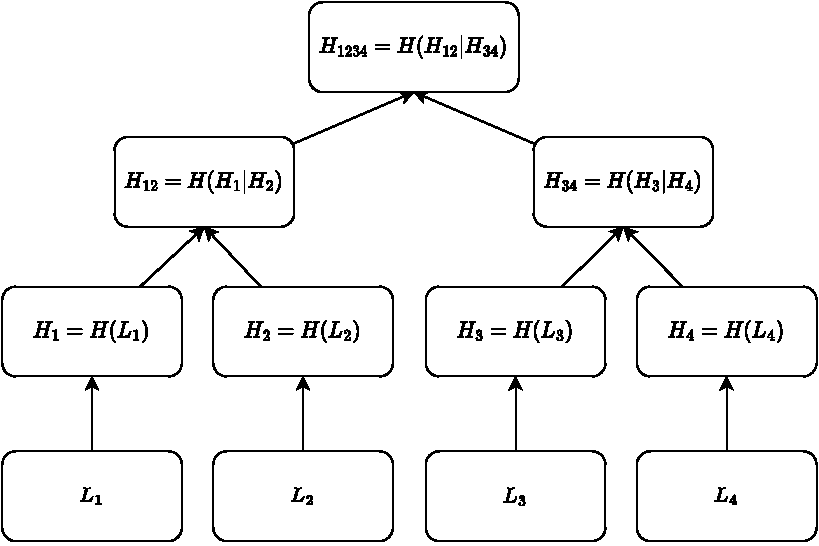
\includegraphics[width=0.6\columnwidth]{\trainingsectiondir/figures/merkle-tree.drawio.pdf}
\caption{Depiction of a Merkle Tree.}
\label{fig:merkle-tree}
\end{figure}

The \textbf{root} represents the overall integrity of all the data in the tree. It is a single hash value that summarizes the entire dataset. If any piece of the original data changes, even a single bit, the \textbf{root} will change significantly.

The \textbf{proving process} for the statement that a leaf node is a part of a given dataset requires computing a number of hashes proportional to the logarithm of the number of leaf nodes in the tree, that is, the number of levels of the tree. More specifically, the proof (often called \textbf{Merkle proof}) consists on the siblings of the path descending to the leaf we want to prove inclusion for. The \textbf{verification process} entails recalculating the hashes within the tree while employing the provided siblings until reaching the root. At this stage, the integrity of the data can be ascertained by comparing the recalculated root hash to the initially provided one.

\paragraph*{Verification Example}

Let's provide an easy example. In the following figure, let's understand how to check if an item exists in a Merkle Tree. Suppose we want to confirm if an element, say, $L_{2}$, is in the tree. To do this, we need two specific hash values $H(L_1)$ and $H_{34}(H_3 \mid H_4)$ to compute the root of the tree $H_{1234}$. If the final root hash matches the one provided to us, it means the element is indeed in the tree. However, if the root hash we calculate doesn't match the expected value, then the element is not in the tree. This simple process helps us verify the presence of items in a Merkle Tree. Observe that we must be given as many hashes as there are levels in the tree, which is  $\mathcal{O}(\log_2(n))$.

\begin{figure}[H]
\centering
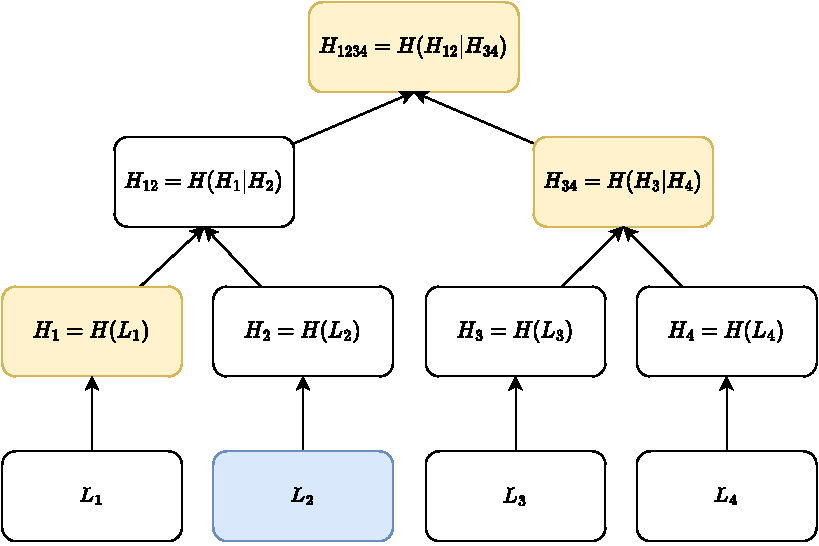
\includegraphics[width=0.6\columnwidth]{\trainingsectiondir/figures/merkle-proof.drawio.pdf}
\caption{The yellow nodes represent the given nodes in the Merkle proof for the leaf node $L_2$.}
\label{fig:merkle-proof}
\end{figure}

If an attacher wants to forge a proof, he needs to find a collision of the hash function, i.e. a different leaf or intermediate node that has the same hash as the one in our tree to have the same root, which is not possible due to the properties of cryptographic hash functions.








%%%%%%%%%%%%%%%%%%%%%%%%%%%%%%%%%%%%%%%%%%%%%%%%%%%%%%%%%%%%%%%%%%%%%%%%%%%
\section{Second Pre-image Attack}

In the previous section, we have presented the concept of a Merkle tree as a secure and efficient procedure to check inclusions. However, a vulnerability known as \textbf{second-preimage attack} emerges if the Merkle hash root is not linked with the tree depth. This scenario allows an adversary to construct an alternative version of the tree, distinct from the one containing the original elements, while yielding an identical Merkle hash root. In Figure \ref{fig:second-preimage-attack-example}, the attacker pretends that elements the elements $h_{01}$, $h_{23}$, $h_{45}$, and $h_{67}$ are the leafs of the tree.

\begin{figure}[H]
\centering
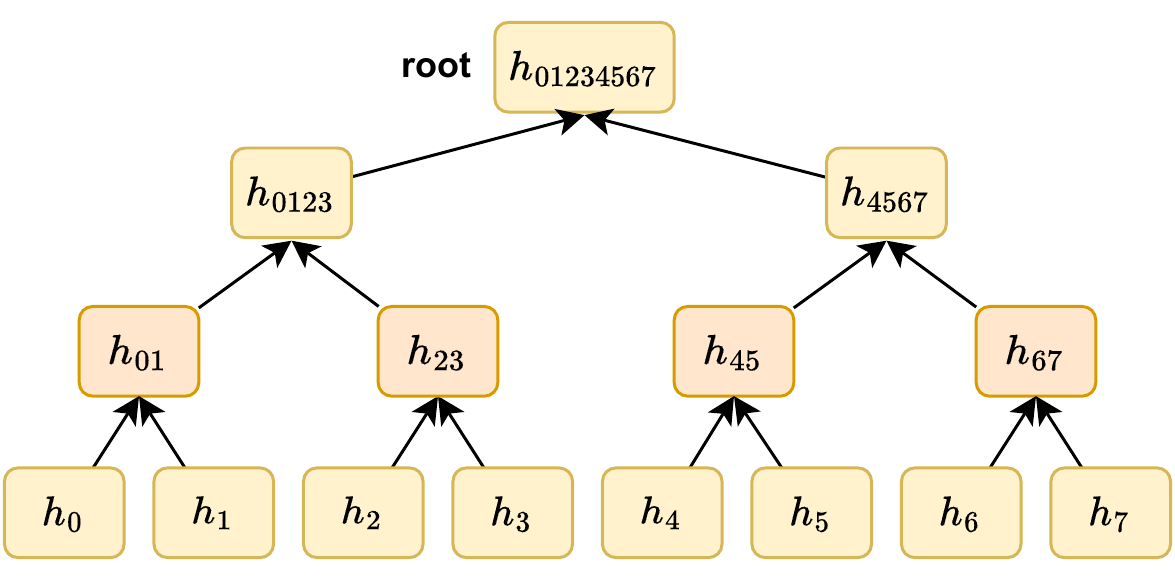
\includegraphics[width=0.6\columnwidth]{\trainingsectiondir/figures/second-preimage-attack.drawio}
\caption{Illustrative Example of a Second-Preimage Attack.}
\label{fig:second-preimage-attack-example}
\end{figure}

An important note is that this attack can occur even if the underlying hash function has no known security weaknesses: it is inherently a problem in how Merkle Tree's are constructed.

In order protect Merkle Trees from second-preimage attacks we can use several techniques:

\begin{itemize}

\item \textbf{Use two different hash functions:}

We can leverage the use of two distinct hash functions, each serving a specific purpose. One of these hash functions is used to calculate hashes for leaf nodes, while the other for branch node hashes. For example, we can prefix a $\texttt{0x00}$ byte to the data before hashing for hashing the leaf nodes, and a $\texttt{0x01}$ byte for hashing branch nodes. This approach allows us to generate two unique hash functions derived from the same underlying design, correctly addressing the issue. In the case of Poseidon (See Section \ref{sec:merkle-tree-zero-knowledge}), it's possible to employ distinct capacity elements to instantiate different hash functions within the same framework. We will denote by $\texttt{H}_0$ and $\texttt{H}_1$ each of the hash functions used in leaf and branch nodes respectively.

\item \textbf{Codify the length of the tree:}

Another approach is to incorporate the length of the tree itself as part of the data being hashed within the leaf nodes. By including the tree length in the hash computation, any alteration with the tree's size (like the one exposed before) becomes immediately evident during verification.

\end{itemize}




%%%%%%%%%%%%%%%%%%%%%%%%%%%%%%%%%%%%%%%%%%%%%%%%%%%%%%%%%%%%%%%%%%%%%%%%%%%
\section{Merkle Tree Classification}

In this section, we will delve into the classification of Merkle Trees by several parameters. To better understand and utilize Merkle Trees, it's essential to classify them based on different criteria. We will explore different ways to group them, considering how they organize data, include data, their shapes, and whether they can be updated or not. Through this classification, we aim to provide a comprehensive perspective on the different types of Merkle Trees and their specific use cases.




\paragraph*{Tree shape}

When classifying Merkle Trees, the shape of the tree is another aspect to consider. The tree shape dictates how nodes and branches are structured within the tree, which can have a significant impact on its efficiency and behavior. Here, we'll explore the two primary dimensions of tree shape:

\begin{itemize}

\item \textbf{Tree's arity:} The concept of the tree's \textbf{arity} refers to the specific number of child nodes that each branch node within the tree can have. Common examples include binary trees, ternary trees, 2-3 trees, hexadecimal trees, and others. Notably, as we will see in Section \ref{sec:ethereum-patricia-trie}, Ethereum's Patricia Merkle Trie employs a hexadecimal tree structure. The arity of the tree significantly impacts the shape of the tree: higher arity produces wider trees meanwhile lower ones produce deeper trees. This also affects the efficiency in several applications.

\begin{figure}[H]
\centering
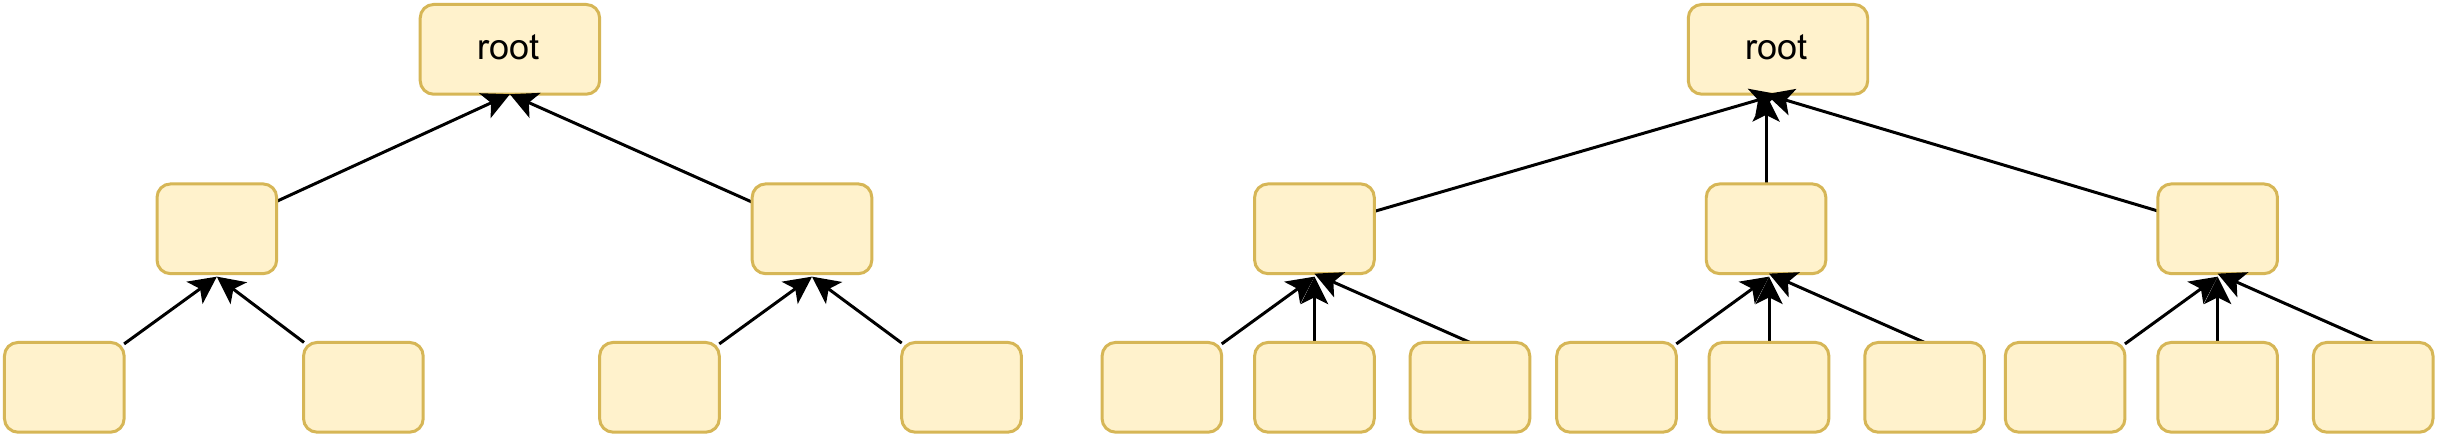
\includegraphics[width=0.80\columnwidth]{\trainingsectiondir/figures/merkle-tree-arity.drawio}
\caption{Binary (left) vs Ternary (right) Merkle Trees.}
\label{fig:merkle-tree-arity}
\end{figure}

\item \textbf{Balanced or unbalanced}: The balance of a tree refers to how its nodes are distributed among its levels. We say that a tree is \textbf{balanced} if the height of the tree is $\mathcal{O}(\log_k n)$, where $n$ is the number of nodes and $k$ is the tree's arity. Balanced trees are often preferred in applications where quick data access and efficient traversal are essential, as they ensure that the worst-case search or verification times are minimized.

\begin{figure}[H]
\centering
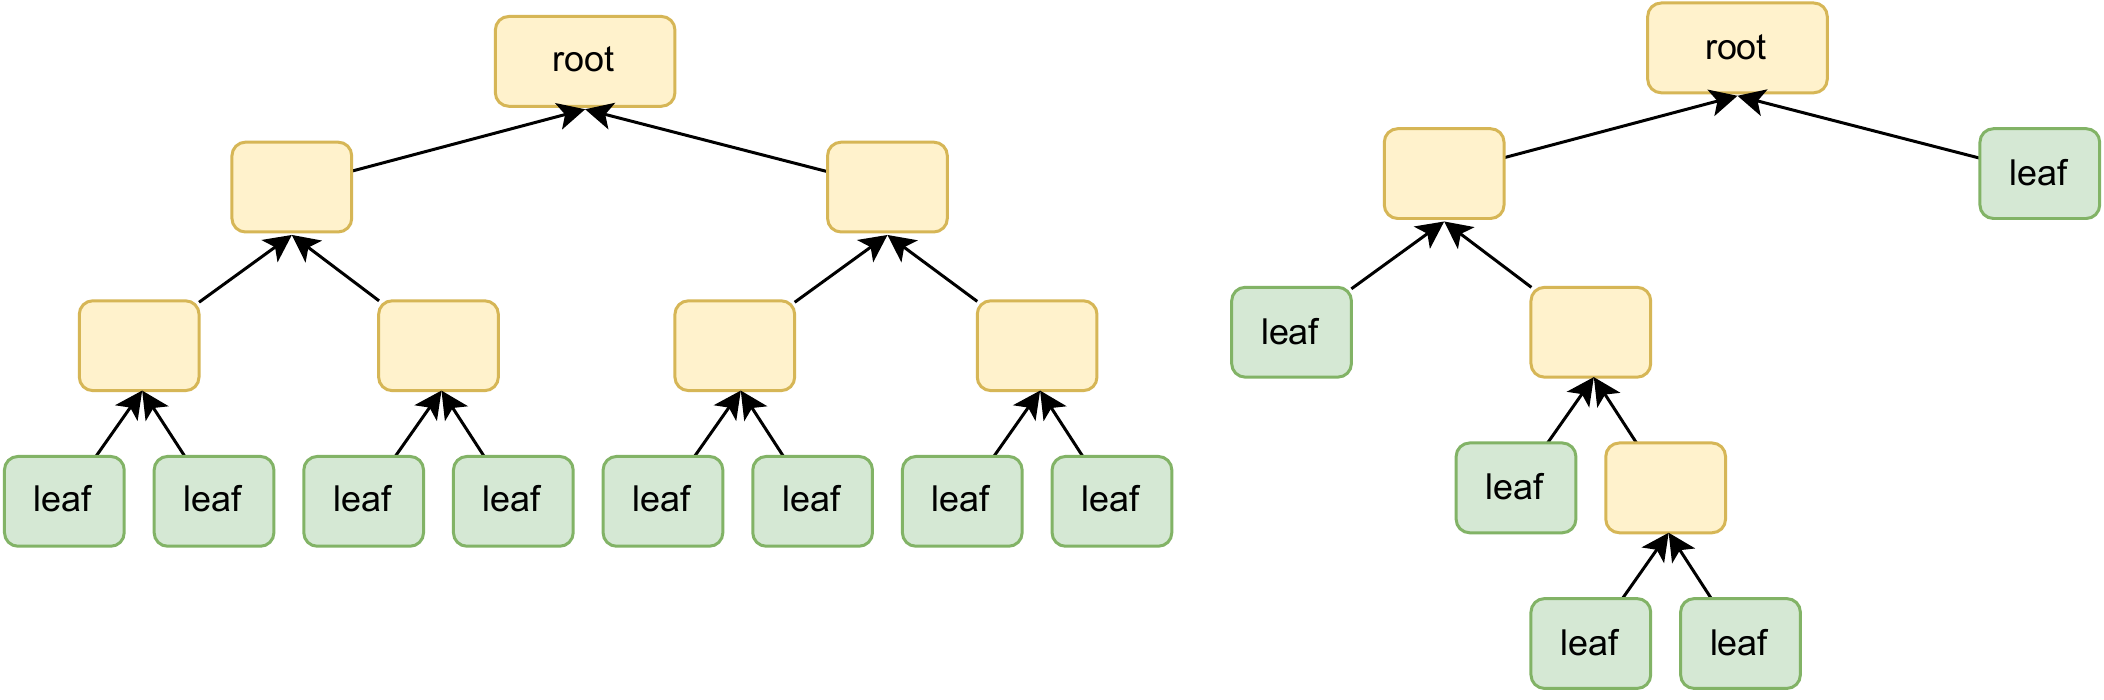
\includegraphics[width=0.80\columnwidth]{\trainingsectiondir/figures/merkle-tree-balancing.drawio}
\caption{Balanced (left) vs Unbalanced (right) Merkle Trees.}
\label{fig:merkle-tree-balancing}
\end{figure}

\end{itemize}




\paragraph*{Data organization}

One of the aspects of classifying Merkle Trees involves considering how the data they store is organized. This organization method will directly impact the tree's applicability. We can distinct two primary categories:

\begin{itemize}
\item \textbf{Unordered:} In this category, there are no specific requirements regarding the arrangement of the data within the tree. Each leaf node represents a data block, but the order of these leafs is completely arbitrary. This lack of order is specially used when the data wanted to be hashed doesn't naturally fit into a specific sequence.

\item \textbf{Key-value:} On the other hand, key-value organized datasets provide a structured approach to data organization. Data within these trees is accessed and indexed using a key. The key determines the position of the leaf node representing the data within the tree. This method is particularly useful when you need to quickly locate specific pieces of data within a larger dataset.

\end{itemize}

\begin{figure}[H]
\centering
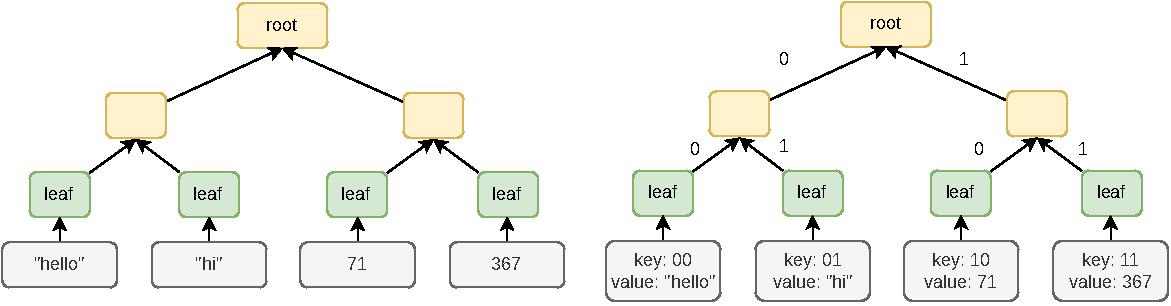
\includegraphics[width=0.8\columnwidth]{\trainingsectiondir/figures/merkle-tree-structuring.drawio}
\caption{Unordered (left) vs Key-Value (right) Merkle Trees.}
\label{fig:merkle-tree-key-value}
\end{figure}



\paragraph*{Data inclusion}

The way Merkle Trees handle data inclusion is another factor in their classification. It determines not only how data is added to the tree but also how the absence of certain data is verified. We can distinct two primary categories:

\begin{itemize}
\item \textbf{Data-inclusion-only:} In this type of Merkle Tree, the only efficient check that we can prove is whether specific data is included in the tree or not. Non-inclusion proofs are still possible but not efficient, breaking Merkle Tree's intention.


\item \textbf{Complete:} In contrast, complete trees also allows non-inclusion proofs, i.e., being able to prove that there is no value associated with a given key. The name complete comes from the fact that these trees store all posible key-value bindings. In this context appears the concept of \textbf{Sparse Merkle Tree (SMT)} which is a complete tree with a hug key space, so it is sparsely populated. The naïve representation of a SMT can have an intractable space (for example, $\mathcal{O}(2^{256}$)) and techniques (such as \textbf{path compression} explained in Section \ref{sec:ethereum-patricia-trie}) to compress the required space are applied to efficiently store the tree. In addition, in SMTs, there is typically a default value (most of the times $0$) that is used when the given key has no value associated.

\end{itemize}



\paragraph*{Updatability}

The category of Merkle tree updatability defines how flexible the tree is in terms of altering its data after its initial construction. This characteristic can significantly impact the tree's functionality and its suitability for different applications. Let's explore the three main categories of Merkle tree updatability:

\begin{itemize}

\item \textbf{Read-only (Non-updatable):} This refers to a tree data structure in which the data or set of elements it represents cannot be altered or updated once the tree is constructed. Essentially, the Merkle tree remains static and immutable.

\item \textbf{Append-only:} In this tree structure, data can only be appended to the existing dataset, it cannot be modified or removed. Therefore, any data added to the tree becomes an immutable part of the tree's historical record. Such limitations provides several optimizations, particularly when it comes to proving insertions within the tree.

\item \textbf{Read-write:} Read-write Merkle trees provide a higher level of flexibility. These trees not only facilitate verification of data integrity but also allows modifications or updates of the underlying data while preserving the tree's structure and retaining its integrity verification capabilities.

\end{itemize}



\section{Storing Ethereum State: Patricia Tree} \label{sec:ethereum-patricia-trie}

The \textbf{Ethereum Merkle Patricia Trie} is a variation of a Merkle Tree and is a fundamental data structure used in the Ethereum blockchain to store and manage the World Ethereum State explained before. In our exploration of Ethereum Merkle Patricia Trie, we will delve into two fundamental concepts: \textit{tries} and \textit{radix tries}. These concepts are crucial in understanding the underlying data structures and mechanisms that power Ethereums World State.

\paragraph*{Tries}

A \textbf{trie} (See Figure \ref{fig:trie-example}), also referred to as \textbf{prefix tree}, is a specialized tree structure used for locating specific keys within a set. Typically these keys are strings, with links between nodes defined not by the entire key, but by individual characters. To access a key, the traversal of the trie occurs in a depth-first manner. This traversal involves following the links between nodes, with each node representing a character within the key.

\begin{figure}[h]
\centering
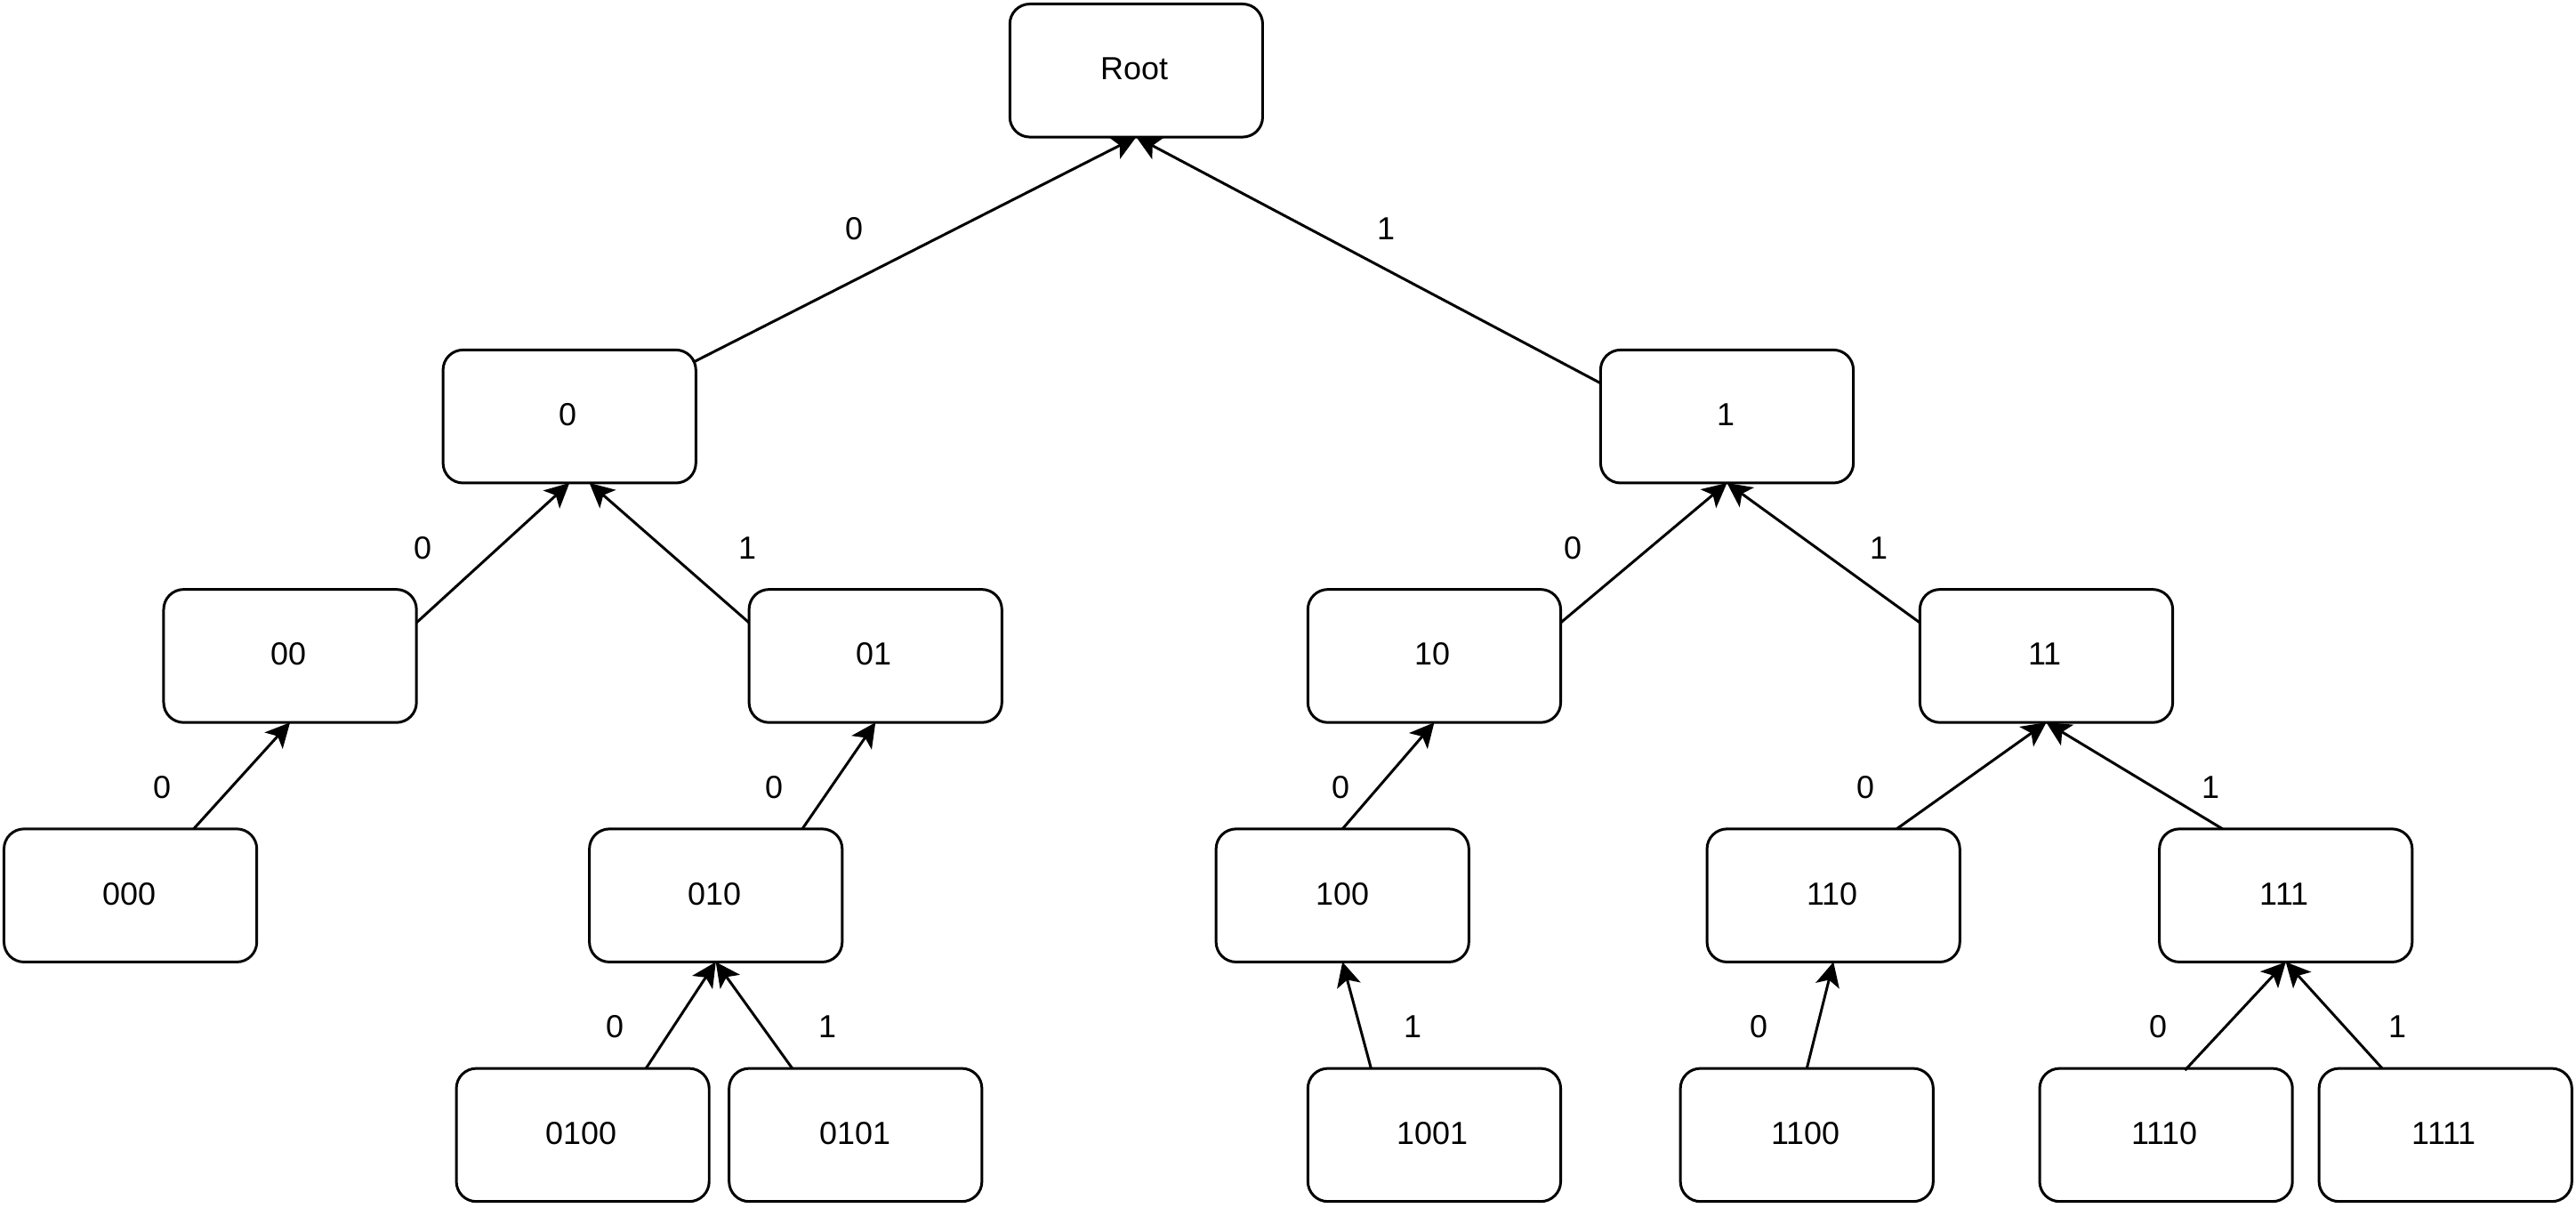
\includegraphics[width=0.75\columnwidth]{\trainingsectiondir/figures/trie-example.drawio}
\caption{We observe how the key of each node is constructed according to its path.}
\label{fig:trie-example}
\end{figure}

\paragraph*{Radix Tries}

A \textbf{radix trie} (See Figure \ref{fig:radix-trie-example}), also referred to as \textbf{compact radix tree}, is a space-efficient data structure that represents a modified form of a trie. Patricia trees were invented by Donald R. Morrisson and named by Donald Knuth, calling them \textit{Patricia's trees} afther the acronym in the title of Morrison's paper: \textit{PATRICIA - Practical Algorithm to Retrieve Information Coded in Alphanumeric}.

In this structure, the \textbf{path compression} technique is used, that is, nodes with a single child are merged with their parent nodes, optimizing space usage. Henceforth, and unlike regular trees, edges can be labelled with sequences of elements as well as single elements. This makes radix trees much more efficient for small sets (especially if the strings are long, which is the case of Ethereum) and for sets of strings that share long prefixes.

\begin{figure}[h]
\centering
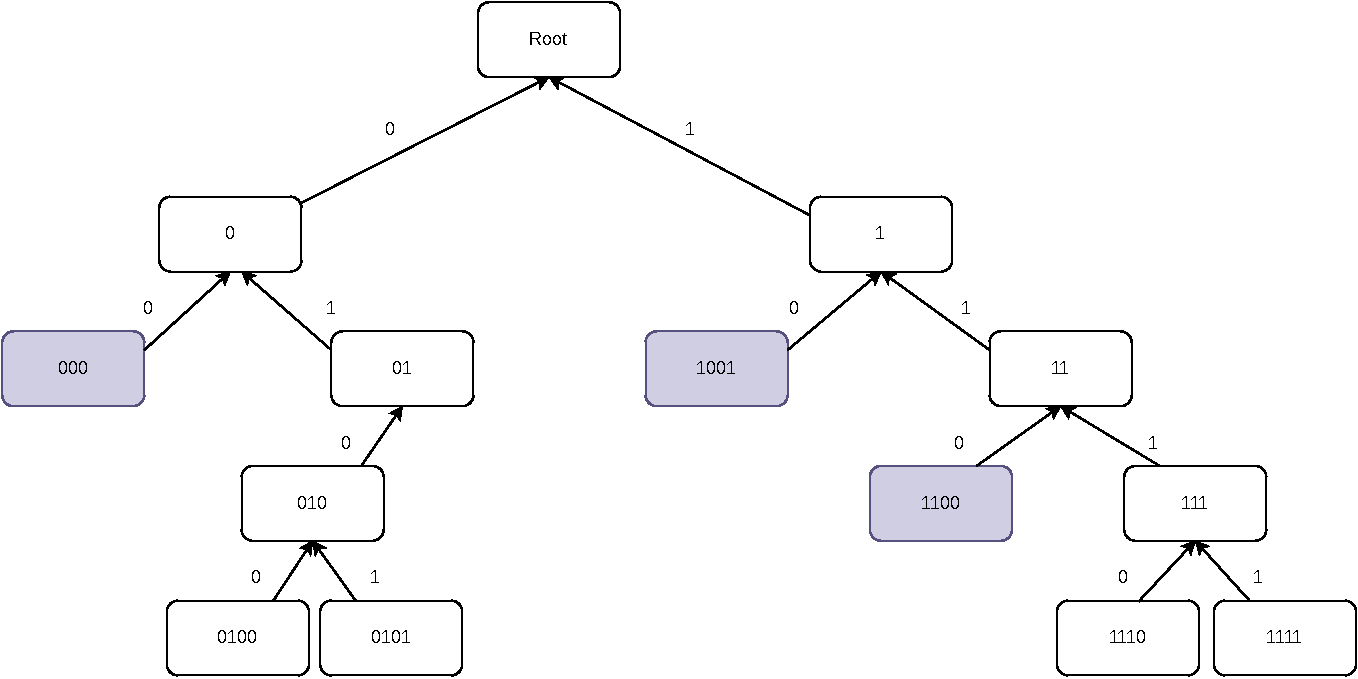
\includegraphics[width=0.75\columnwidth]{\trainingsectiondir/figures/radix-trie-example.drawio}
\caption{The purple boxes represent the nodes whose path could be compressed because their chain was redundant.
}
\label{fig:radix-trie-example}
\end{figure}


\paragraph*{The Ethereum Merkle Patricia Trie}

Ethereum's Patricia Trie uses a 16-ary radix trie structure and it is sometimes called a hexadecimal trie. The trie is used to store the state of Ethereum accounts. As explained before, this includes their \texttt{balance}, \texttt{nonce} together with \texttt{codeHash} and \texttt{storageRoot} in the case of Contract accounts. The root of each of them is stored in the blockchain's block header, making it possible to verify the state of the system at any given block.

The tree is built by linking nodes using deterministically-generated cryptographic hash digests. More specifically, the key of an specific \texttt{ethereumAddress} is always computed as its \texttt{keccak256} hash:
\[
\texttt{keccak256(ethereumAddress)},
\]
meanwhile the value (whose hash will be included in the tree as a leaf) is always obtained applying the Recursive-length prefix serialization (a.k.a \texttt{rlp}) of the $4$ item consisting on the $4$ stored elements specified before:
\[
\texttt{rlp([nonce, balance, storageRoot, codeHash])}.
\]
Observe that, \texttt{storageRoot} is also the root of another Patricia trie which: the \textbf{storage trie}.
%maybe say "Note that \texttt{storageRoot} serves as the root for another Patricia trie, specifically the \textbf{storage trie}."
 Storage trie is where all contract data lives. Unlike the previous one, there is a separate storage trie for each account.

To look up a value in the Patricia Tree, you start at the root and traverse the tree by following the appropriate child node at each level based on the hexadecimal digits of the key. This process continues until you reach the leaf node that contains the desired data.

As we have seen, this particular Merkle Tree is a critical component of the Ethereum blockchain's data structure, enabling efficient and secure storage and retrieval of the system's state. Nevertheless, the hash function employed by Ethereum's Patricia Tree is not ideally suited for zero-knowledge settings, like a zk-Rollup. In this scenario, we opt for the Poseidon hash function, as we explain in the next section. Moreover, in the context of zero-knowledge, it's more efficient to adopt a binary tree structure. This approach sidesteps the need for additional constraints and significantly reduces costs. The Patricia Tree involves a costly 16-node hash to level up, while the binary tree employs a more economical two-node hash.







%%%%%%%%%%%%%%%%%%%%%%%%%%%%%%%%%%%%%%%%%%%%%%%%%%%%%%%%%%%%%%%%%%%%%%%%%%%%%
\section{Merkle Trees for Zero Knowledge Proofs} \label{sec:merkle-tree-zero-knowledge}

When building Merkle trees for enabling Zero-Knowledge proofs about data being included or not in the tree, there are some additional aspects that need to be considered:

\begin{itemize}

\item \textbf{Algebraic Natura of Zero-Knowledge Hash Functions:}

Unlike classical hash functions, which tend to be bit-oriented, those employed in Zero-Knowledge protocols possess a distinctive algebraic nature. This algebraic structure facilitates a seamless arithmetization process.

\item \textbf{Data and Field Size Discrepancies:}

One of the challenges arises from the disparities between the size of the data intended for storage in the tree and the size of the underlying field used by the Zero-Knowledge system. To solve that, we can adopt a \textit{limbs-like strategy}, strategically partitioning and processing data into field sized \textit{limbs}, ensuring compatibility between data and the underlying cryptographic field.

\item \textbf{Determinism in Zero-Knowledge:}

Determinism is fundamental in Zero-Knowledge protocols and, hence, all the operations and parameters within the tree must be deterministic, meaning they yield predictable results for a given set of inputs.

\item \textbf{Constraints on Operations:}

The operations and parameters governing the tree must be meticulously constrained at the time of constructing the proofs. Carefully defining and limiting the operations prevent potential vulnerabilities and attacks, making the arithmetization sound.

\end{itemize}

\paragraph*{Suitable Hash Function for Zero-Knowledge}

%TODO: Maybe we not include this here

%TODO: Maybe we not include this here

\texttt{Poseidon} is a cryptographic hash function that has garnered attention for its unique properties and suitability in the context of Zero-Knowledge proofs. It was originally designed to address some of the limitations and challenges faced by traditional hash functions in this specific application domain. From now on, we will consider an instantiation of \texttt{Poseidon} over a Goldilocks field (that is, $\FF_p$ where $p = 2^{64} - 2^{32} + 1$), that takes as entry $8$ field elements divided into two groups: four of them are know as \textbf{capacity elements}, and the other $4$ are the elements to be hashed, known as \textbf{input elements} and outputs $4$ field elements known as \textbf{output elements}. We will denote a Poseidon hash as follows:

\[
\texttt{Poseidon}(\texttt{capacity};\texttt{values})
\]

Here, $\texttt{capacity}$ is an array of $4$ field elements representing the capacity elements, and $\texttt{values}$ is an array of $4$ field elements representing the inputs of the hash. Observe that we can also see \texttt{values} as an array of $8$ (almost) $32$-bits elements. In our context, two instances of Poseidon hash function are employed for protecting the tree against second-preimage attacks: $\texttt{Poseidon}(0; \cdot)$ for branch nodes and $\texttt{Poseidon}(1; \cdot)$ for leaf nodes.







%%%%%%%%%%%%%%%%%%%%%%%%%%%%%%%%%%%%%%%%%%%%%%%%%%%%%%%%%%%%%%%%%%%%%%%%%%%
\section{A zk-Friendly Sparse Merkle Trie for the zkEVM State}

The Merkle tree we are using to store the zkEVM State is a Sparse Merkle Binary Trie fully updatable (that is, allowing both read and write operations)  used to represent key-value data. We will also make it radix in order to optimize storage space. Due to its construction, it will be unbalanced by nature (since keys, which are used to completely locate leaves within the tree, will be hashes of some data).

\paragraph*{A Glimpse Through Toy Example}

Let's visualize the tree using an example. Lets suppose we have some set of data associated with four keys: \texttt{000110}, \texttt{001011}, \texttt{001100}, and \texttt{101101}. Prefixes are used to position the leaves containing data. We have four distinct prefixes: \texttt{000}, \texttt{0010}, \texttt{0011}, and \texttt{1}. Recall that zero nodes are used to signify the absence of keys under a given prefix. With this design, similar keys share a common path in the tree, saving space.

\begin{figure}[H]
\centering
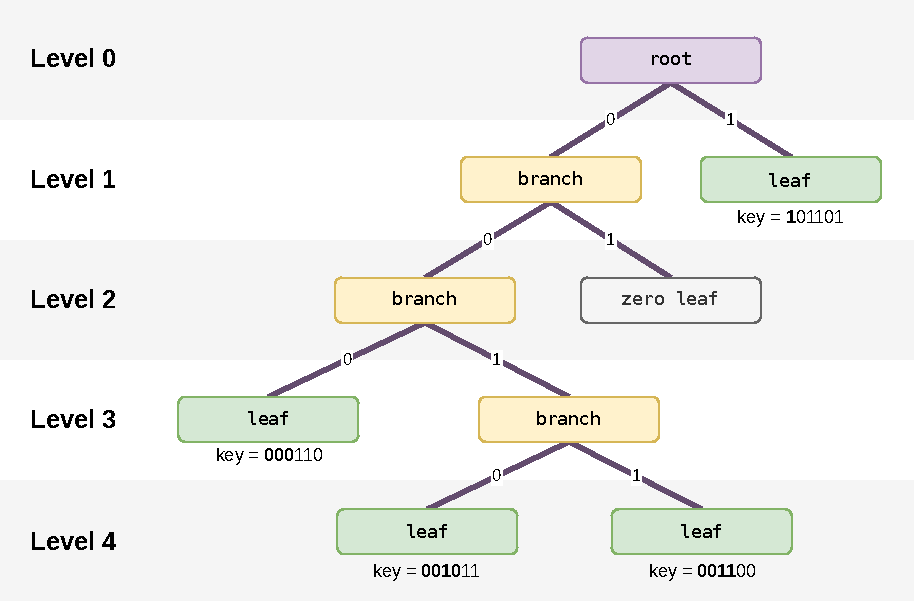
\includegraphics[width=.8\columnwidth]{\trainingsectiondir/figures/smt-trie.drawio}
\caption{Illustrative Example of a Sparse Merkle Trie.}
\end{figure}

\paragraph*{The Four Node Types} In the proposed example we can see the $4$ different types of nodes appearing in our tree design:

\begin{itemize}

\item \textbf{Root node}: The root node is the top node of the tree, the only one node at level zero, connecting all branches and leaves. It is the starting point for traversing the tree structure. It serves as a cryptographic summary of all the tree, the final hash of the entire dataset.

\item \textbf{Leaf node}: Leaf nodes encapsulate the actual data associated with a key. Its stored value can be obtained by hashing unique information of each key-value binding of the dataset.

% Explain what we are hashing exactly.

\item \textbf{Branch node}: Branch nodes serve as intermediaries within the tree structure, positioned at various levels between the root node and the leaf nodes. These nodes actively guide the traversal path within the trie. The primary responsibility of a branch node is to store the hash derived from concatenating the hashes of its two child nodes. This hash encapsulates the segment of the cryptographic summary representing the data contained in the subtree rooted at that branch node.

\item \textbf{Zero node}: Zero nodes \textbf{do not} represents a zero value for a specific key. Instead, they denote the absence of a subtree beneath a branch node. In our example, we can see that all keys starting with $01$ share the default value of $0$. Consequently, there is no need for these keys to be individually present as nodes in the tree, and this is where zero nodes come into play. However, the tree actually stores several keys starting with $00$. These keys require the presence of a branch node at level $2$ to obtain the parent's node hash. The optimization lies in the decision not to hash the subtree below with hashes of zero but rather to represent it with an explicit zero value. In practical terms, this means that the branch node at level $1$ assumes a specific value:
\[
\texttt{H}_0(\texttt{leftChildNode}, 0).
\]

This optimization is called \textbf{partial tree construction}.

\end{itemize}



%\newpage
%\bibliographystyle{alpha}
%\bibliography{../bib/bibliography}

\newpage
\appendix

\end{document}